%!TEX root=report.tex
\subsection{GMM clustering}
\label{section:result-gmm}

Like with K-means clustering, a matrix $X$ with dimensions ($64800 \times 341$) is used. Due to the high number of variables in GMM, the dimensionality was reduced using PCA and only selecting the first 10 PCs.
The results were not ideal, so instead a kernel version of PCA was used.

\begin{itemize}
\item The first 10 principal components were used
\item The ``Radial basis function'' was used as a kernel function
\item The amount of degree is 3
\item The gamma coefficient is set to $\sfrac{1}{341}$
\end{itemize}

\begin{figure}[H]
	\center
	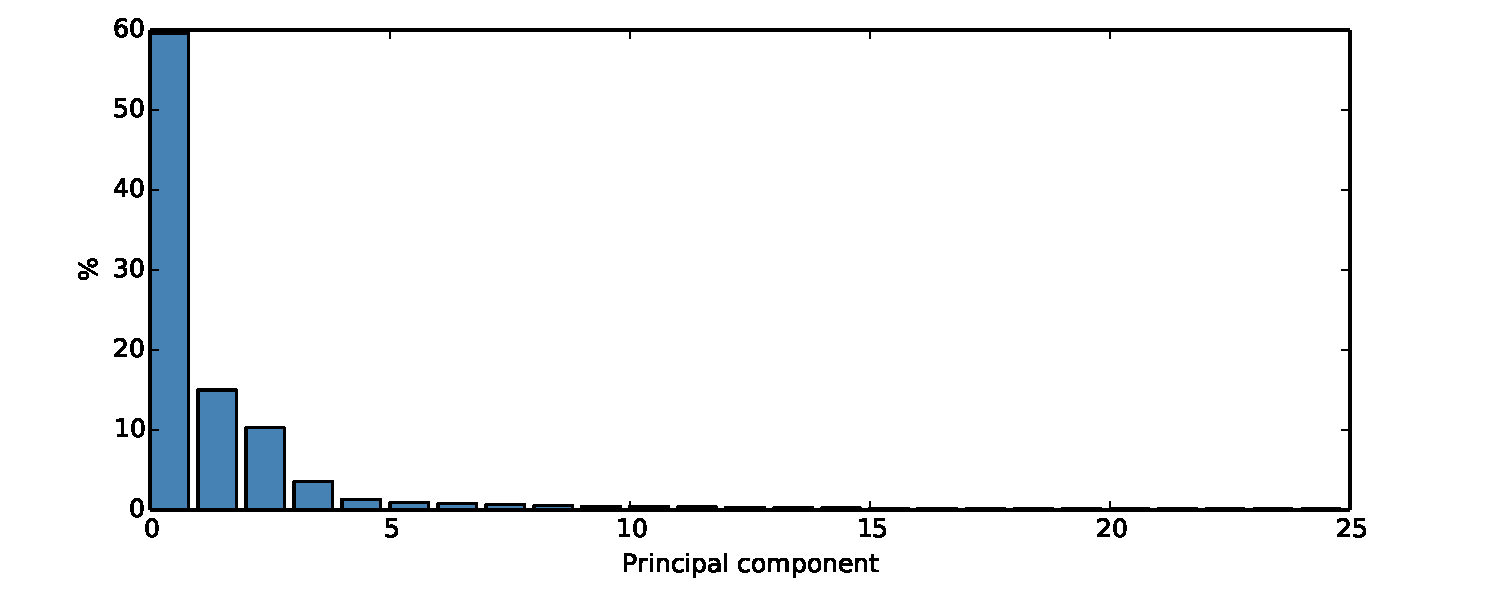
\includegraphics[width=\textwidth]{figures/gmm-pca-explaned}
	\caption{Variance explained for the first 25 PCs, calculated as eigenvalues in $K = H(X) H(X)^T$.}
	\label{fig:gmm-pca-explaned}
\end{figure}

As seen in Figure \ref{fig:gmm-pca-explaned}, by selecting the first 10 PCs 93.18\% of the variance in the data (in the kernel space) is explained.

Next the GMM with 6 clusters was computed using the projected data. 
\begin{figure}[H]
	\center
	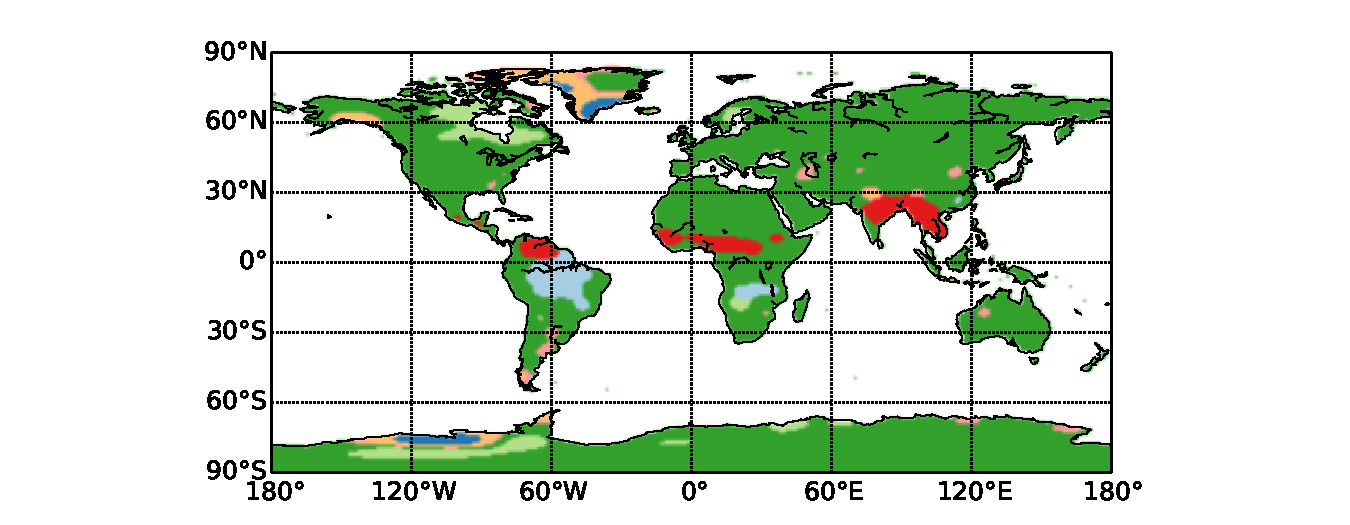
\includegraphics[width=\textwidth]{figures/gmm-world}
	\caption{Each position is a point, the color then matches a given cluster.}
\end{figure}

\begin{figure}[H]
	\center
	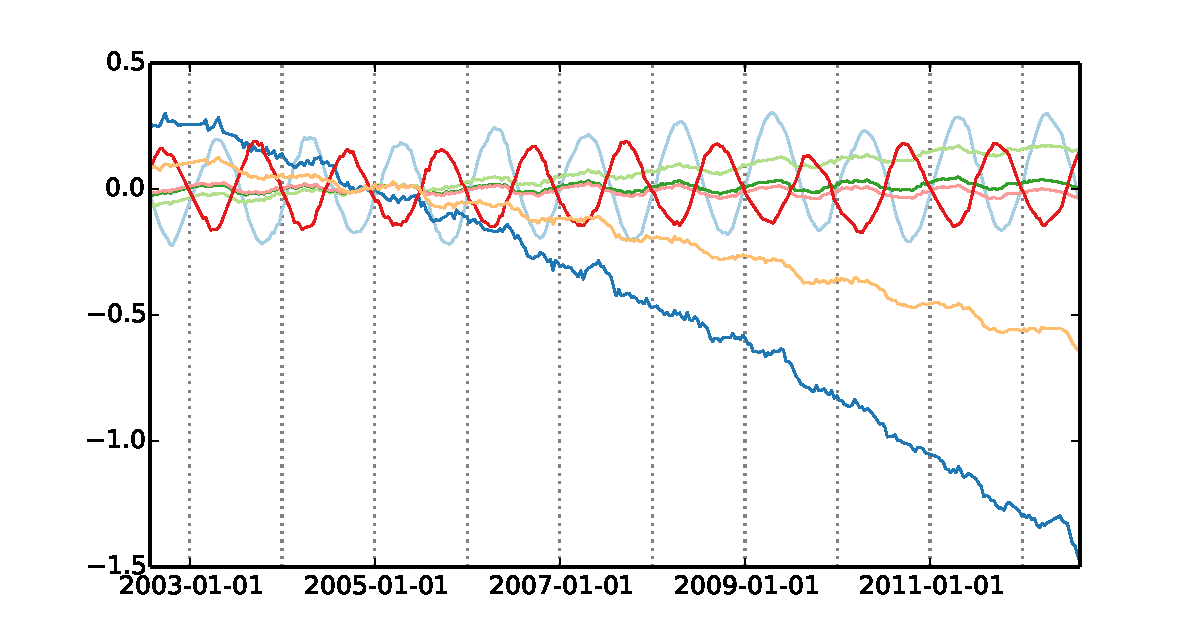
\includegraphics[width=\textwidth]{figures/gmm-centroids}
	\caption{The mean vectors for each Gaussian component, projected back in the original space, using the inverse kernel PCA transformation.}
\end{figure}

Comparing the two plots above:
\begin{itemize}
	\item Light green have a slight mass increase, this was also seen in K-means clustering. Since this is observed in North America, it is likely caused by post glacial rebound.
	\item  Red and light blue correlates with extreme and regular seasonality, also very much like K-means.
	\item Blue and orange correspond with trending mass loss. With the same locations as in K-means.
	\item The big difference between GMM and K-means, is that the world graph is a lot less noisy. Only those positions with a significant different behavior than normal (green) have been caught by GMM.
	\item Finally the pink cluster is almost not noticeable and could be considered redundant. 
\end{itemize}
